\chapter{Data Productions}

Data analysis is a highly dynamic activity $-$ particularly for a nascent, large-scale experiment. As a result, having a flexible and scalable data management and analysis framework is of particular importance. Different data components may be needed at different points of study, brand new readouts may be added in the middle of data taking, and analysis styles themselves may differ from user to user -- all of which are either facilitated or impeded, depending on the flexibility of the framework implemented.

In an attempt to provide such a framework to its users, SeaQuest makes use of the capabilities of an array of MySQL servers, leveraging relational database technologies. While MySQL and database systems are nothing new, even to physics experiments, they are not widely adopted among the physics community. Often, in the cases that they are, the resulting product tends to be ineffective or inefficient. 

During my tenure at SeaQuest, I was primarily in charge of the effort to decode the raw, serialized data from the data acquisition systems and store them in a manner in which it could be readily accessible by collaborators worldwide. Beyond that, an emphasis was placed on curating the tracked physics data and preparing it in such a way that facilitates quick and simple analysis from many different analytical software packages. 

In this chapter, the details regarding the processes and formats that define the online and offline data productions will be described in some technical detail. The technologies used to perform this were a combination of compiled C/C++ codes, MySQL, ROOT, and the Fermilab Computing Division's primary computing grid. The end product provided to all collaborators was in the form of unified ``schemas'' (or, groups of tables) possessing all of the combined \emph{run, spill, event, slow control}, and \emph{tracked} information, along with specific data quality flags in place to assist in the selection of good, analyzable data. Finally, there is a retrospective discussion on the scalability and best practices, followed by speculation on how future data management technologies might be used at SeaQuest and other experiments.

\section{Raw Data Processing}

The three raw outputs of the data acquisition systems, as described above (and in Chapter 2) are Main DAQ CODA files, Scaler DAQ CODA files, and Beam DAQ ASCII files. Each raw data file corresponds to the data taken from certain subsystems over approximately one to two hours of running time. These three types require varying degrees of de-serialization, parsing, processing, and storage -- a process as a whole defined as \emph{decoding}. 

All raw data files are backed up to long-term tape storage (managed by FNAL Computing Division), and the decoded and processed data gets stored on one of four MySQL servers to be used for analysis by the collaboration. Data is also output to ROOT files for ease of use by independent tracking programs and those who prefer navigating data in the raw ROOT TTree format.

\subsection{CODA Event Format}

A single CODA file can be described as being a chain of events. These can generally be divided into ``CODA Events'' for those related to the CODA file itself, and ``Standard Physics Events'' when containing experimental data read out by CODA and its subsystems. Each event can be represented by an array of unsigned 32-bit integers. When using the CODA EVIO (event input/output), one whole event is read out into such an array, which can vary in size from 6 to $\sim50,000$ integers long, depending on the type of content.

CODA Events primarily correspond to the actions taken by a shift-taker using the \emph{rcgui} application on the data acquisition computer. The types of events that fall under this category are Sync, Prestart, Go, Pause, and End. It should be noted that the Sync and Pause events do not generally get used at SeaQuest. These provide markers in the CODA file of what commands were given to CODA through the course of taking data. 

Before data taking can begin the readout controllers and the trigger supervisor need to be loaded with a designated firmware in order to operate properly. Before a CODA file is started and created, this ``Download'' is performed, and then CODA is ready to transition from the downloaded state to the prestarted state. The CODA file is then initialized with a prestart event, whose format can be seen in Figure~\ref{fig:coda-prestart-go}. The most important information stored in the prestart event is the run number, which is used universally through the experiment. 

Once in a prestarted state, a ``Go'' action is initiated to transition it into data taking mode. This action generates a Go event. If ever paused, a Go event would be created once data taking was resumed. Go events contain the current time and the number of events in the run so far, also seen in Figure~\ref{fig:coda-prestart-go}. It should be noted that the ``time'' stored in these events is not trusted, as the data acquisition computers are not synced to an official external source.

\begin{figure}
	\centerline{
		\mbox{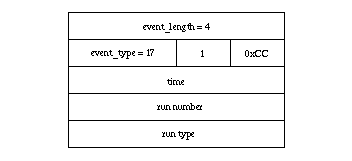
\includegraphics[width=0.5\textwidth]{figures/production/prestart_event.png} 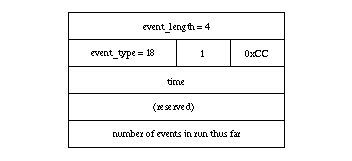
\includegraphics[width=0.5\textwidth]{figures/production/go_event.png}}
	}
	\caption{(Left) The Prestart event, with event type 17; (Right) The Go event, with event type 18\cite{jlab:coda}.}
	\label{fig:coda-prestart-go}
\end{figure}

The last CODA Event of importance is the End Event. This contains the number of events in the run, but primarily serves as a marker to any programs reading the CODA file that the EOF (end of file) has been reached, and to commence any post-run processes.

Most of the events in the CODA file, however, will be ``Standard Physics Events''. The contents of these can be varied, but can be characterized generally as having a header containing the total length of the event (in number of 32-bit integer ``data words''), followed by several ``data banks'', which are typically filled with a series of ROC outputs (Fig.~\ref{fig:coda-physics-roc}). The contents and formats of the ROC data banks are completely controlled by the ROC programming, and whatever set of 32-bit words the ROC has to read out, it will store in its ``data words'' block. 

\begin{figure}
	\centerline{
		\mbox{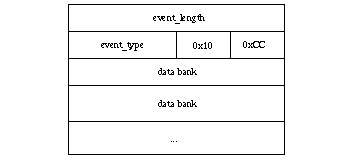
\includegraphics[width=0.5\textwidth]{figures/production/physics_event.png} 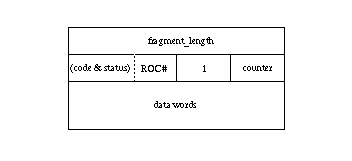
\includegraphics[width=0.5\textwidth]{figures/production/roc_event.png}}
	}
	\caption{(Left) A standard physics event, with various event types, filled with a series of data banks; (Right) The ROC data bank format\cite{jlab:coda}.}
	\label{fig:coda-physics-roc}
\end{figure}

\subsection{ROC Data Bank Formats}

The data within the ROC data banks have their own definition of encoding, and it differs from event type to event type. Of the types most commonly used, there are scaler, QIE, slow control, and ``JyTDC'' formats. These formats were designed and implemented gradually and as-needed through the development of the SeaQuest data acquisition. Through these iterations, there was a consistent effort spent devising an output format for the TDCs that was as compressed as possible while performing very quickly (to reduce deadtime). 

The first TDC format devised was compact, but required some computation and caused unnecessary dead time. After that, signals were encoded into a non-zero-suppressed format where a binary string such as \verb|00011111111110000| would represent a signal, with each \verb|1| representing \unit[2.5]{ns} of contiguous signal. This then required writing too much data, which still caused some dead time, and the file size of the raw data would become bloated. Eventually, a quick, compressed, complex format called ``JyTDC2'' was adopted and became the standard for the MainDAQ encoding.

\subsection{Decoding Raw Data}

The CODA file decoding process is nearly identical in the cases of the Main DAQ and Scaler DAQ outputs, and only differ by content; the Scaler DAQ reads out specific scaler data, and the MainDAQ contains TDC readouts of the detectors. For each one to two hour \emph{Run}, the CODA files can be well-described as the following sequence of events (and the data they contain):
\begin{enumerate}
	\item Prestart Event (Run data)
	\item Begin Spill Event (Spill data, Scaler readout)
	\item Many Physics Events (Event data, TDC readout)
	\item End Spill Event (Spill data, Scaler readout)
	\item SlowControl Event (Slow control readout, Spill ID readout)
	\item Spill Counter Event (Spill ID readout) \newline ...(Repeat 2-6 for each \emph{Spill})
\end{enumerate}

The decoding programs use C and C++ in conjunction with Jefferson Lab's CODA I/O library\cite{jlab:coda} to read these events and parse them according to their individual formats. Data from these CODA events are decoded and placed into hierarchical categories.

\subsubsection{Run Level Data}

Run-level data contains data and metadata pertaining to the entirety of the run that is recorded. At the time of the Prestart Event, the date and time of the run are stored, along with a readout of the specific settings of all non-trigger TDC boards. Settings regarding which triggers are enabled and what each of their prescale factors is also stored in the run-level data.

After the End Event is encountered, metadata is aggregated and stored regarding such items as the number of chamber hits, the types of triggers that were fired, the target positions used, average magnet currents, and other useful metrics. All of these fields of settings and aggregated values can be used later on to quickly determine if a run is analyzable, or if it has characteristics that are desirable for specific niche analyses.

\subsubsection{Spill Level Data}
The \emph{Beginning of Spill} (BOS) and \emph{End of Spill} (EOS) events bookend the set of physics events for a given spill. At each BOS and EOS events, the 140 MHz VME scalers are read out. At the beginning of the spill, all scalers are zeroed out, and then read out again after the spill has ended.

Slow Control events are read out between spills, which contain data regarding the current spill identifier number, target systems, beam and radiation monitors, and environmental readings.

The spill identifier (\emph{spillID}) is what is used to synchronize the data together across various data acquisition systems. As such, the \emph{spillID} is read out redundantly in both Slow Control and Spill Counter events (which contain only the \emph{spillID} value) to ensure that the data is appropriately labeled.

When the End Event (for the whole CODA file) is reached, the independently-recorded Beam DAQ data (recorded in an ASCII file) is read and stored with the rest of the Spill-level data.

\subsubsection{Event Level Data}\label{sec:event-data}
For each spill, $\sim3k$ events are triggered to be recorded, though this number can vary greatly with the particular beam settings of a run. With each event, three types of information are stored: the trigger which fired the event, a measure of the beam intensity per RF bucket, and the full detector readouts. The detector readouts require the most processing of all the rest of the data. The CODA files contain the hardware addresses of each detector \emph{hit}, along with a \emph{TDC time}. The following steps briefly summarize the processing steps:
\begin{enumerate}
	\item Mapping: Map the hardware address to a detector name and detector element number
	\item Timing: Classify hits as in-time or not and calculate \emph{drift time} from TDC time
	\item R-T (time-to-space): Translate \emph{drift time} to \emph{drift distance}
	\item After-Pulse Elimination: Remove hits that result from signal reflection and other electronic artefacts
	\item Trigger Road Reconstruction: Use \emph{v1495} TDC hits to reconstruct possible trigger roads that may have fired
	\item Hodoscope Masking: Remove drift chamber hits that have no adjacent hodoscope hit
	\item Trigger Road Masking: Same as hodoscope masking, but only using hodoscopes from reconstructed trigger roads
\end{enumerate}
This fully processed data is then stored into one the experiment's MySQL databases and/or a ROOT file.

%%%%%%%%%%%%%%%%

\section{Online and Offline Production Processing}

There are two running modes of raw data processing: on-line and off-line. These are designed to suit two needs: (1) the need to monitor the experiment and the detector readouts, and (2) to perform a full analysis of the data taken.

\subsection{Online Monitoring and SeaScape}

For the on-line mode of productions, all Run- and Spill-level data is decoded, but only 1-in-$n$ Physics Events are processed, where $n$ is typically between 3 and 15, depending on the event data taking rates. This \emph{``sampling mode''} is used in order for the decoding to reliably keep up with even high-intensity beam data. This data pipeline is important for on-line monitoring of the experiment by shift crews. With this up-to-the-minute stream of data, any abnormalities in features such as duty factor, wire maps can be observed directly and acted upon quickly.

In 2014, Dr. Sylvester Joosten, a then-UIUC PhD student working on the HERMES experiment, collaborated with SeaQuest to create a robust, responsive web page for online monitoring. This project, named \emph{SeaScape}, was built using JavaScript, Python Flask, and used a Python MySQL API for database interfacing and data handling. The result of the combined efforts was a full-featured, globally-available, password-protected web app hosted on a Fermilab virtual server. Current capabilities of SeaScape consist of wire maps (histograms of hits) for all groups of detectors (Fig.~\ref{fig:seascape-wiremaps}), time series of ScalerDAQ, BeamDAQ and Slow Control (Fig.~\ref{fig:seascape-targpos}) values, and even a note-taking section for use by those observing remotely or those on shift. 

Any run schema may be selected for displaying, and two distributions from two different schemas may be compared against each other. A spill selection slider bar is provided so that a user may step through the data for various ranges of spills. An export feature is provided for users to output the displayed figures to PDF files.

\begin{figure}
	\centering
	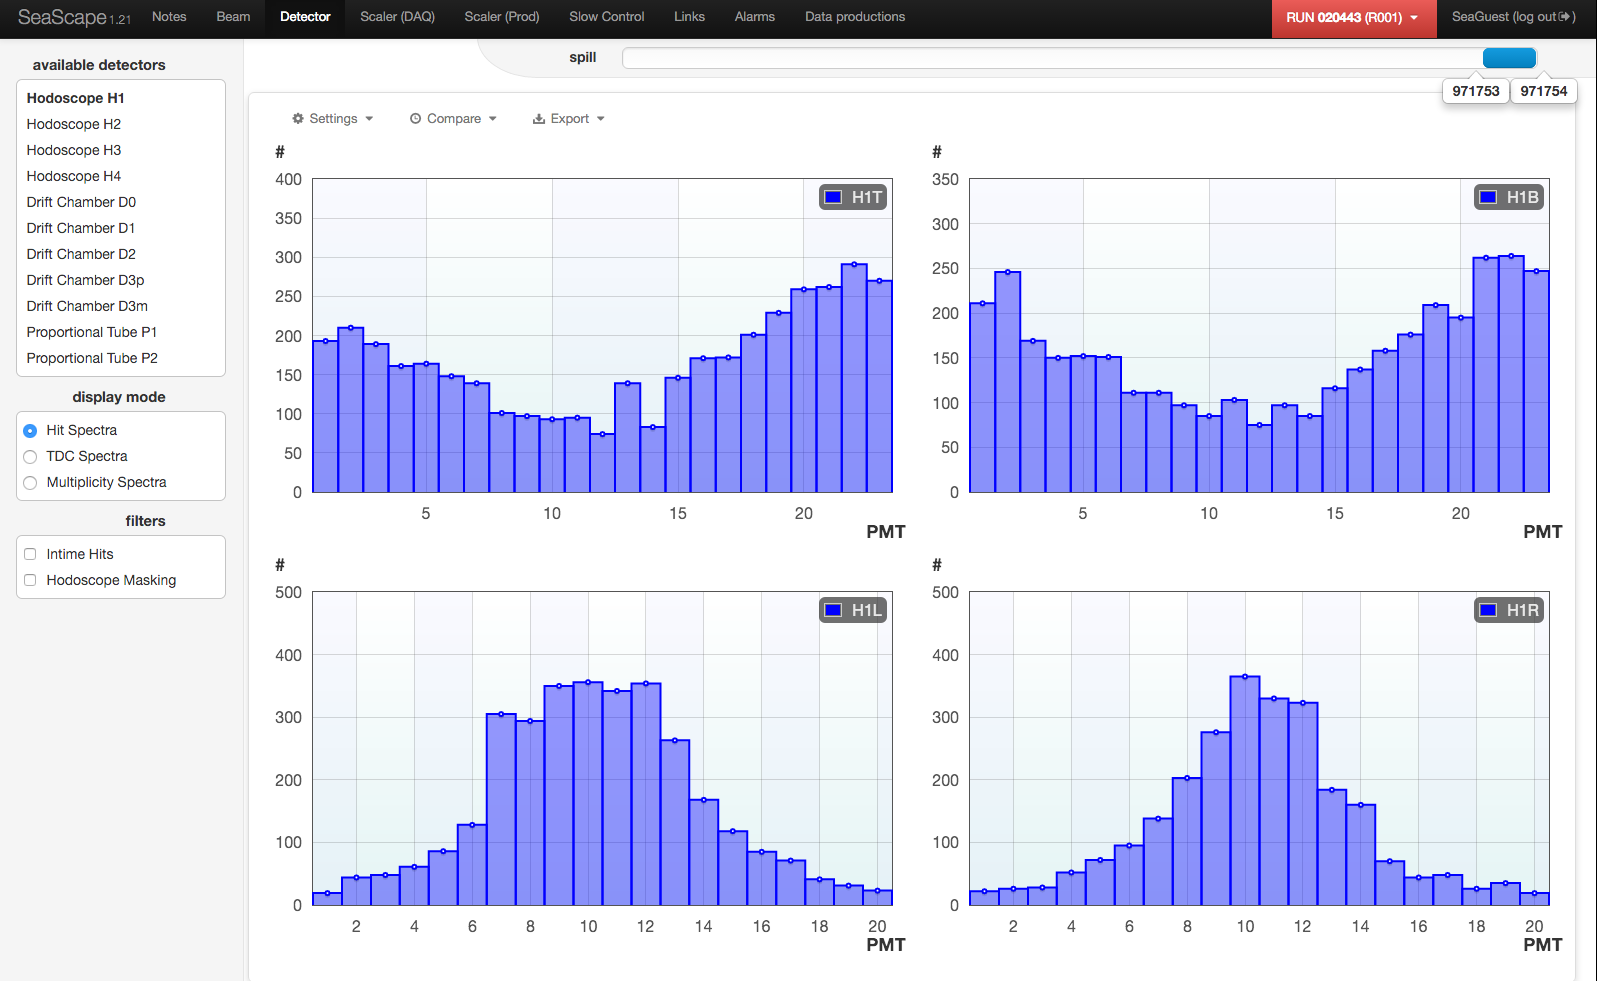
\includegraphics[width=\textwidth]{figures/production/SeaScape-wiremap.png}
	\caption{The SeaScape Online Monitor displaying the hit distributions for the Station 1 hodoscopes. Run selection is in the top red button selector, and the Spill selection is in the bar just below the top.}
	\label{fig:seascape-wiremaps}
\end{figure}
\begin{figure}
	\centering
	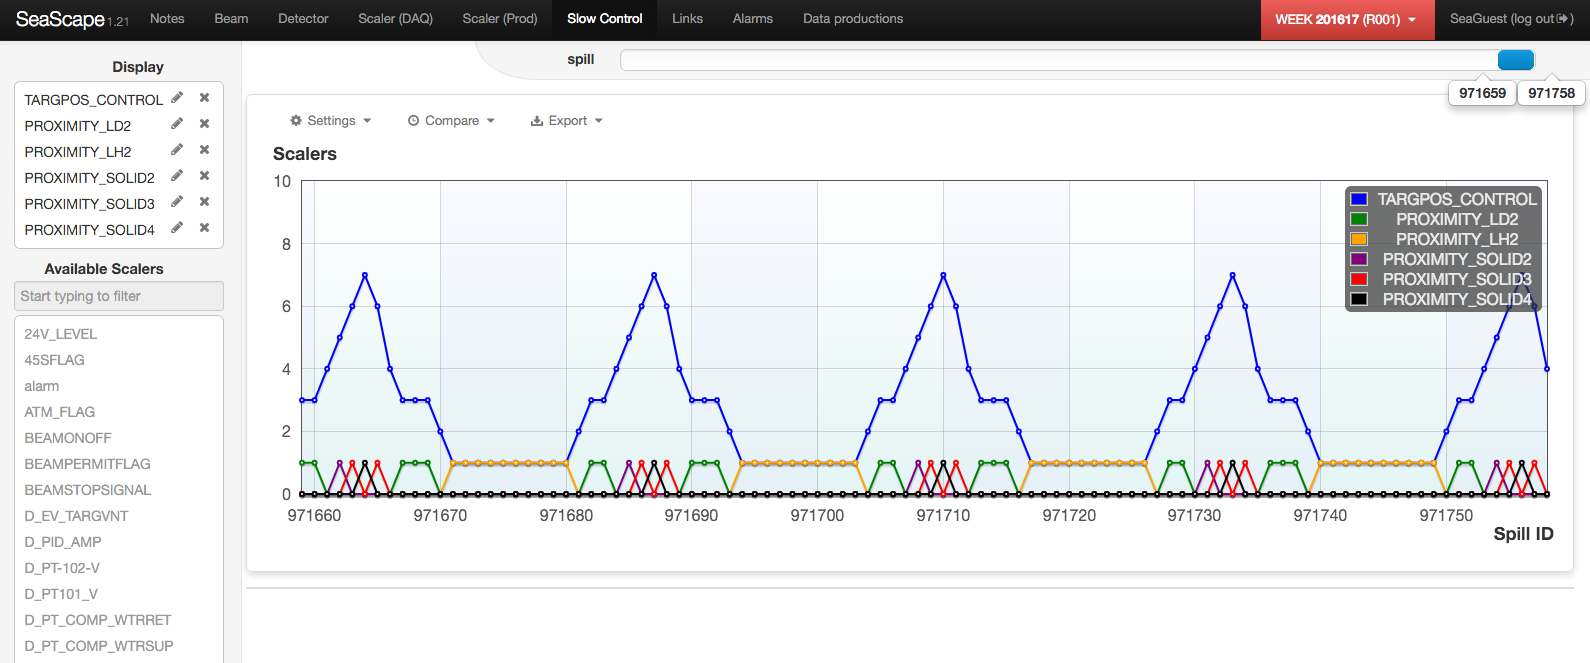
\includegraphics[width=\textwidth]{figures/production/SeaScape-targPos.png}
	\caption{SeaScape displaying target position data for a sequence of spillIDs. Up to six different values can be shown at once against each other (scale-able for easier comparison) on each of the Slow Control, BeamDAQ, ScalerDAQ pages.}
	\label{fig:seascape-targpos}
\end{figure}

\subsection{Offline Batch Processing}

For off-line, or ``batch'', productions, a large group of categorically similar runs is defined, and the chain of production processing is initiated. The steps of this process are generally emph{decoding, tracking, archiving, and merging}. The logical blocks of runs are typically defined by ``roadset'', or, the version of the set of trigger roads used in the L1 trigger matrix. Differences in these trigger matrices can affect the distributions to a degree commensurate with the difference in the set of roads that are triggered on by the FPGA-1 trigger. As such, each block of data using a given roadset should be analyzed individually and then have its results combined with those of other roadsets via a weighted average.

The decoding and tracking are performed on Fermilab Computing Service's FermiGrid, which provides the computing resources necessary to process hundreds of runs simultaneously. The tracking has also expanded its capabilities to run on the Open Science Grid, which is a grid computing network that pools together computational resources from national laboratories and universities throughout the world\cite{osg:doc}. This allows the intensive reconstruction algorithms to perform its tracking on thousands of grid nodes at once.

A single decoding job submission will output the processed data to one of the four available MySQL servers and also to a ROOT file. The processed data in ROOT form at this stage is called the ``digit'' data. Whether or not the decoding sends Hit and TriggerHit information to the MySQL schemas is an option that can be set at the time of batch processing. The current operating mode is to perform batch processing, sending Hit/TriggerHit data to MySQL for only 1-in-50 runs. This allows users to capture a glimpse of full hit distributions for runs within a roadset while preventing a single pass of the experiment's data from filling up all available data storage space.

After this step, jobs will be submitted to run one or both of the two tracking programs based on the ROOT file and/or the MySQL data. Once the tracking is completed, the ROOT file is archived on the Fermilab BlueArc NAS backup system for storage and for tracking.

Upon the completion of decoding and tracking of a specified range of runs, all of their Run-, Spill-, and Event-level data, along with its tracked data, is combined into a single \emph{merged} schema. These \emph{merged} schemas are mirrored across all four of the MySQL servers for optimal redundancy and availability.

\section{RDBMS Data Structure}

The processed data is primarily stored in MySQL Server 5.1 databases. MySQL is an open-source \textbf{R}elational \textbf{D}ata\textbf{b}ase \textbf{M}anagement \textbf{S}ystem (RDBMS) developed by Oracle that is well-suited for the storage and responsive querying of hierarchical data.

\emph{Why was SQL chosen for the data storage?} The ease of use in querying and the flexibility were important factors here. Querying using the Standard Querying Language (SQL) provides an English-readable (and thereby easier-to-learn) way to formally ask the database for what you're looking for. Flexibility stems from the ability to \emph{update} existing data with best-known calibrations and the ability to modify the structure of the stored data \emph{in situ}. \emph{Why MySQL of all the SQL technologies?} The short answer there is speed and support. There are several RDBMS to choose from, but at the time of deciding in 2010, MySQL had exhibited a slight speed edge over most of the competition (such as PostgreSQL). What truly made the decision was the near-universal support that both Oracle and all other languages supported MySQL. Nearly every coding and analysis language out there supports an interface to MySQL.

Each run is decoded into its own schema and contains its own instances of all tables of a specified design. The tables are all \emph{join}-able to each other by sharing \emph{foreign keys} with each other in the form of the \emph{runID}'s, \emph{spillID}'s, and \emph{eventID}'s. The contents of the tables are \emph{indexed} in such a way that \emph{joins} and queries gain a speed performance boost, but this comes at the cost of disk space.

\subsection{Querying Language}

The data on the server is world-wide accessible and can be queried using SQL, which is styled very much like a logical, readable sentence, and therefore has a relatively shallow learning curve as compared to other programming languages. For instance, in order to select the eventID, spillID, and dimuon vertex ($dz$) position from the \emph{kDimuon} table for cases where $4.2 \leq M_{\gamma^*} \leq \unit[10]{GeV}$, one need only execute the query:
\begin{lstlisting}
SELECT eventID, spillID, dz
FROM kDimuon
WHERE mass BETWEEN 4.2 AND 10;
\end{lstlisting}
where whitespace is added only for readability and the query keywords are capitalized, but not case-sensitive.

The key benefit of using a relational database is in relating two tables. Any two tables can be \emph{joined} on each other via overlapping fields, and that total result itself can be joined again. In the following query example:
\begin{lstlisting}
SELECT dimuonID, dpz, SQRT(POW(dpx,2)+POW(dpy,2)) AS dpt, mass, costheta, dutyFactor53MHz
FROM kDimuon
INNER JOIN Spill USING(spillID)
INNER JOIN BeamDAQ USING(spillID)
WHERE 
mass BETWEEN 4.2 AND 10 AND
Spill.dataQuality = 0;
\end{lstlisting}
exhibited are the following actions and features:
\begin{itemize}
	\item The kDimuon table is joined to the Spill table using the common spillID field
	\item An ``INNER JOIN'' is one in which the joined field must have matching values in both tables in order to return a value
	\item The kDimuon-Spill joined result is, in turn, joined on the BeamDAQ table (again sharing the spillID field) to gain access to the associated duty factor field
	\item The SQL math library is used (SQRT() and POW()) functions) to calculate $p_T$ from dpx and dpy
	\item On-the-fly renaming of fields (here, ``dpt'' is the name given to a calculated field)
	\item Use of the Spill data quality criteria discussed in depth in Section~\ref{sec:dq}
\end{itemize}
And so with a modest familiarity with SQL and knowledge of what tables exist and what fields exist in what tables, an analyzer is able to very quickly put together a query to access a very \emph{specific} set of data that they are looking for. For more on SQL, tutorials, how-tos~\cite{ww3school}, and very well-supported documentation from Oracle~\cite{oracle:mysql} are ubiquitous online for anyone wishing to pick up this language in a short amount of time. 

What's more, there is very broad support for interfacing with SQL servers in general (programming APIs), and so the resultset of the queries can be funneled directly into any analysis code in any programming language due to the large array of MySQL API's available. This was one of the key factors in choosing SQL to host the analysis data. Those wishing to use ROOT, Excel, Mathematica, Matlab, R, or Python could do so, using a single interfacing language to access the data.

\subsection{Atomic Data Schema}

With a basic knowledge of the standard querying language, one then only needs to know where to find what data in order to query it. A summary of the atomic schema layout can be found in Figure~\ref{fig:schema-layout}. For every run that SeaQuest takes, when it is fully processed, a schema is created with all of the tables listed in this figure. While the raw data tables have already been sufficiently discussed in the previous sections, some new tables are the calibration tables (used to perform all the timing and mapping mentioned in Section~\ref{sec:event-data}), the BeamDAQ table which is directly uploaded from the BeamDAQ output, the Slow Control data which is the categorized data read out from the EPICS server, and the Tracked Data which is uploaded directly by the tracking software.
\begin{figure}
	\centering
	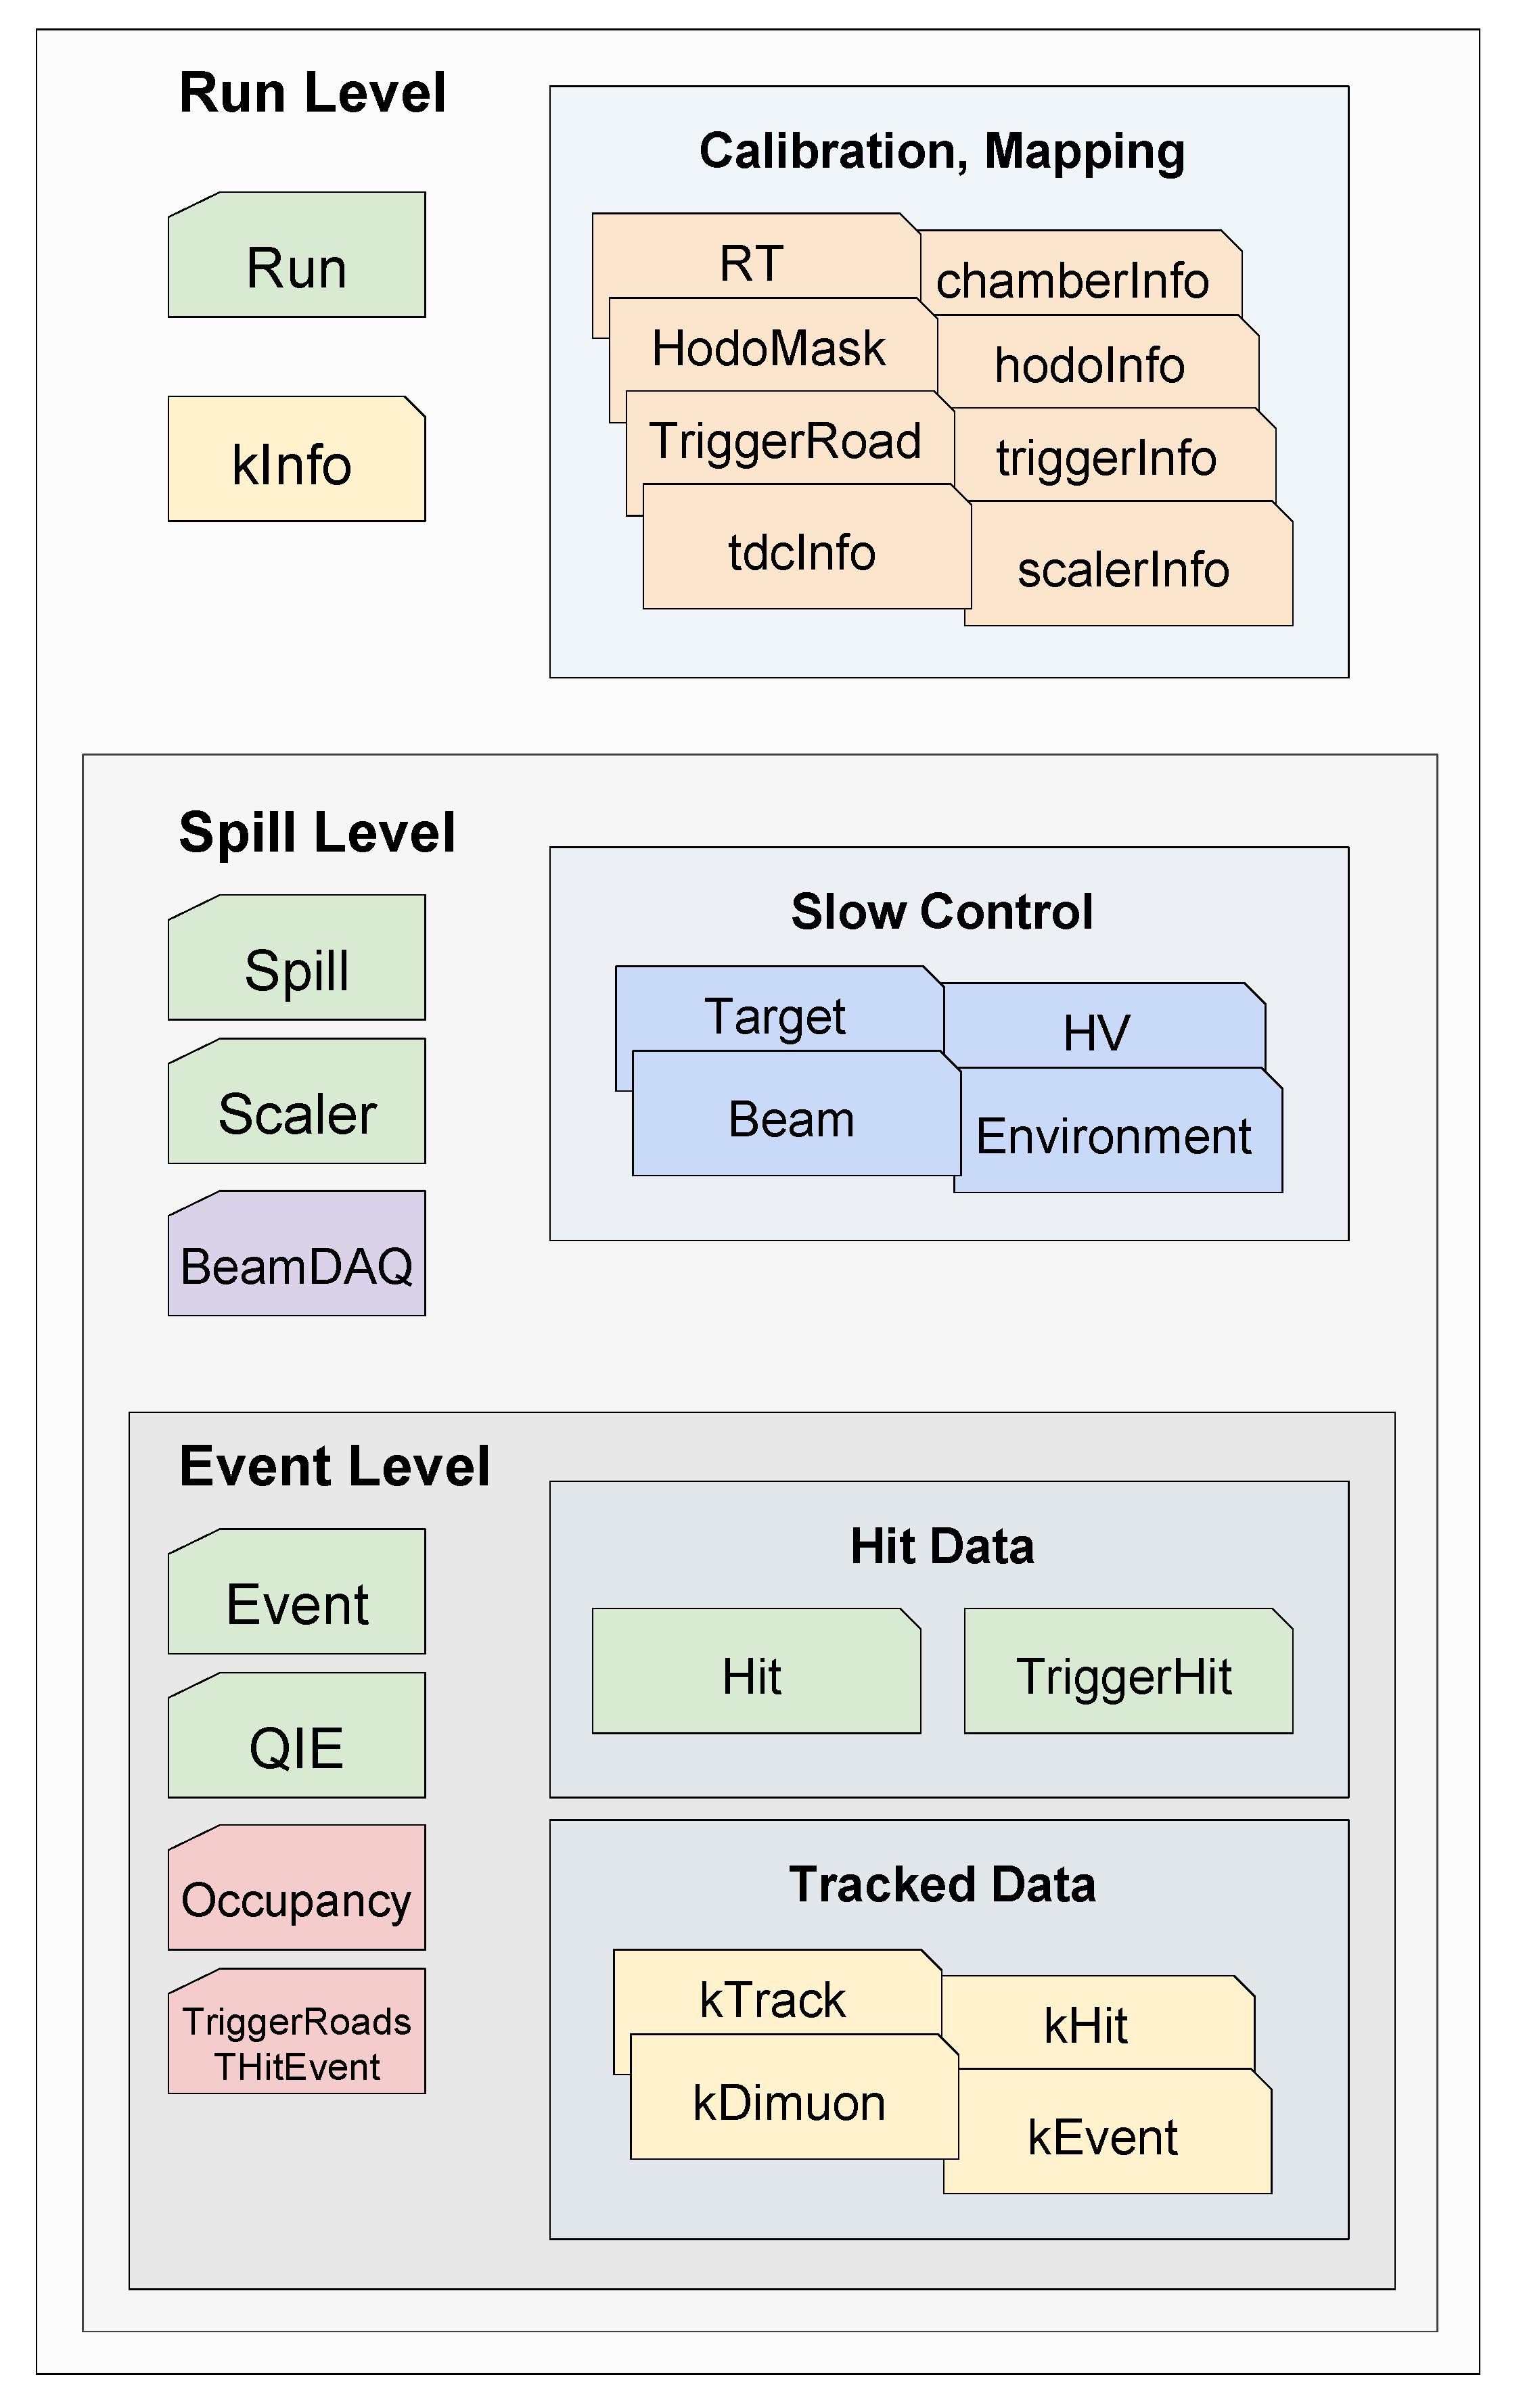
\includegraphics[height=0.9\textheight]{figures/production/Schema-Layout.pdf}
	\caption{A visualization of the hierarchy and categorization of the data stored in the MySQL tables at SeaQuest. Data can be grouped into Run, Spill, and Event hierarchies, and categorized into raw data (green), calibrations (orange), BeamDAQ data (purple), slow control data (blue), reconstructed data (yellow), and aggregated metadata (red).}
	\label{fig:schema-layout}
\end{figure}

\subsection{Production Management}

Without a naming scheme, a database environment can become untenable as no one will know where to find what they're looking for. A set of prefixes and a template for standard run schema names were advised so that as little referential material would be needed as possible. The schemas kept on the servers are grouped into the following:
\begin{itemize}
	\item \textbf{run\_XXXXXX\_RYYY}: \emph{XXXXXX} is the 6-digit, zero-padded run number, \emph{YYY} is the 3-digit, zero-padded production revision number. All runs decoded, processed, and tracked keep their data in these schemas.
	\item \textbf{merged\_roadsetXX\_RYYY\_VZZZ}: \emph{XX} is the 2-digit trigger roadset version number, \emph{YYY} is the aforementioned production revision number, and \emph{ZZZ} is the version of the merged production. This is the aggregated analyzable data from a large ($\sim1000$) number of runs combined into a single set of tables.
	\item \textbf{mc\_*}: The prefix used for Monte Carlo simulated data. Naming conventions defined and kept self-consistent by the Monte Carlo production manager.
	\item \textbf{geometry\_*}: The prefix used for experiment geometry definitions and survey numbers. Naming conventions defined and kept self-consistent by the geometry production manager.
	\item \textbf{user\_*}: A prefix reserved for users to create, store, and manipulate their own data freely.
\end{itemize}

As table definitions were revised and new standards were imposed for the standard \emph{run}-level productions, the production revision number was incremented (e.g. \emph{R003, R004, R005}). As new tracking results were generated and new \emph{merged}-level definitions were imposed, the merged version number was incremented (e.g. V001, V002, V003). Users are encouraged to keep their own tables of signal dimuons for their own analysis in their own user\_\emph{username\_descriptive\_name} schemas for some analytical permanence that doesn't require re-running of their full analysis codes.

\section{Data Quality}\label{sec:dq}

In Section~\ref{sec:data-cuts}, the number of data quality cuts is substantial. Over the course of analysis, many small issues were discovered that required a check for. Many of these values and criteria would change from roadset to roadset. As a result, performing a data quality check on the data became very cumbersome and error-prone for analysts. It was proposed to simply remove the bad quality data from the tables, but there were certain circumstances where users might with to \emph{relax} some of the criteria. As a result, the use of a bit pattern, or bitmask, was implemented to summarize the data quality classifications. 

\subsection{Bit Pattern Fields}

A single 32-bit integer can be represented as a string of 32 \verb|0|s and \verb|1|s when represented in binary. With a bit pattern defined, each of these can act as a flag for \verb|0| meaning ``passed the quality check'' and \verb|1| meaning ``failed the quality check.'' With this being the case, it becomes a simple matter to select data which passes all data quality criteria by requiring \verb|dataQuality = 0|, since any check failing will cause the entire integer to be non-zero.

This also allows users to relax criteria by use of bit-wise logic. If we have an 8-bit data quality word, and the 3$^{rd}$ data quality bit ($2^3=8$) is \verb|1| (\verb|0b00001000|), but we wish to relax the criteria for the 3rd bit, one could still select the data that passes all other checks with a bit-wise \emph{and} and a \emph{twiddle} operator:
\begin{lstlisting}
~0b00001000 = 0b11110111
0b00001000 & 0b11110111 = 0b00000000
\end{lstlisting}
So, in practice, if we want to relax the 3$^{rd}$ bit criteria (\verb|0b00001000 = 8|), then in place of a \verb|dataQuality = 0| cut, one would add a \verb|dataQuality & ~8 = 0|.

\subsection{Spill Data Quality}

Within the Spill table, there is a field named ``dataQuality'', which is a 32-bit integer. Many of the 32 bits have been defined to reflect certain Spill quality criteria that were summarized in Table~\ref{tab:spill-cuts}. Blocks of bits are reserved for certain categories of quality checks such as ``Beam,'' or ``DAQ/Trigger,'' though a data quality criteria have not been assigned to every bit. The Spill dataQuality bit pattern definition can be found in Table~\ref{tab:spill-dq}.

\begin{sidewaystable}
	\centering
	\begin{tabular}{llllllll}\toprule
		N$^{th}$ bit & Category & Description & Roadset 57 \& 59 & Roadset 61 & Roadset 62 & Roadset 67 & Roadset 70 \\\midrule
		0 & Beam & Duty Factor & [15,60] & [15,60] & [10, 60] & [10, 60] & [10, 60] \\
		1 & Beam & G2SEM &[2e12, 1e13] & [2e12, 1e13] & [2e12, 1e13] & [2e12, 1e13] & [2e12, 1e13] \\
		2 & Beam & QIEsum & [4e10, 1e12] & [4e10, 1e12] & [4e10, 1e12] & [4e10, 1e12] & [4e10, 1e12] \\
		3 & Beam & FMAG Current & $>$ \unit[1000]{A} & $>$ \unit[1000]{A} & $>$ \unit[1000]{A} & $>$ \unit[1000]{A} & $>$ \unit[1000]{A} \\
		4 & Beam & KMAG Current & $>$ \unit[1000]{A}  & $>$ \unit[1000]{A} & $>$ \unit[1000]{A} & $>$ \unit[1000]{A} & $>$ \unit[1000]{A} \\
		5 & Beam & Undefined & & & & & \\
		6 & Beam & Undefined & & & & & \\
		7 & Beam & Undefined & & & & & \\
		8 &  Target & Undefined Targ. Pos. & & & & & \\
		9 & Target & Targ. Pos. & $\in [1,7]$ & $\in [1,7]$ & $\in [1,7]$ & $\in [1,7]$ & $\in [1,7]$ \\
		10 & Target & Undefined & & & & & \\
		11 & Target & Undefined & & & & & \\
		12 & Target & Undefined & & & & & \\
		13 & Target & Undefined & & & & & \\
		14 & Target & Undefined & & & & & \\
		15 & Target & Undefined & & & & & \\
		16 & DAQ / Trigger & Inhibit & [4e9, 1e11] & [4e9, 1e11] & [4e9, 2e11] & [4e9, 2e11] & [4e9, 2e11] \\
		17 & DAQ / Trigger & Busy & [4e9, 1e11] & [4e9, 1e11] & [4e9, 1e11] & [4e9, 1e11] & [4e9, 1e11] \\
		18 & DAQ / Trigger & AcceptedFPGA1 & [1e3, 8e3] & [1e3, 12e3] & [1e2, 6e3] & [1e2, 6e3] & [1e2, 6e3] \\
		19 & DAQ / Trigger & AfterInhFPGA1 & [1e3, 3e4] & [1e3, 1e6] & [1e2, 1e4] & [1e2, 1e4] & [1e2, 1e4] \\
		20 & DAQ / Trigger & Accepted/AfterInh & [0.2, 0.9] & [0.0, 0.9] & [0.2, 1.05] & [0.2, 1.05] & [0.2, 1.05] \\
		21 & DAQ / Trigger & TSGo & [1e3, 8e3] & [1e3, 12e3] & [1e2, 6e3] & [1e2, 6e3] & [1e2, 6e3] \\
		22 & DAQ / Trigger & BOS and EOS exist & & & & & \\
		23 & DAQ / Trigger & MATRIX1 Settings & & & & & \\
		24 & Decoding & Duplicate values & & & & & \\
		25 & Decoding & Missing values & & & & & \\
		26 & Decoding & Problematic Spill Range & & & & & \\
		27 & Decoding & Undefined & & & & & \\
		28 & Decoding & Undefined & & & & & \\
		29 & Decoding & Undefined & & & & & \\
		30 & Decoding & Undefined & & & & & \\
		31 & Decoding & Undefined & & & & & \\ \bottomrule
	\end{tabular}
	\caption{The Spill table dataQuality bitpattern definition.}
	\label{tab:spill-dq}
\end{sidewaystable}

\subsection{Other Data Quality Bits}

The dataQuality bits paradigm is used on the Event- and Hit-level data, though to a lesser extent. At the event-level, there are cases where the QIE experiences a readout error, and there is no intensity information for that event as a result. There are also cases in which the v1495 TDCs experience an error, and there is no capability to perform the precise ``RF in-time'' flagging using the triggering hodoscopes and their RF timing. The 0$^{th}$ bit has been reserved for indicating events with excessively high occupancy in any one detector group, but no consensus could be reached regarding how high of an occupancy was too large. As of now, the bit is reserved but unused.

For the Hit-level, requiring \verb|Hit.dataQuality=0| will return all hits that are (0) in the in-time window, (1) are masked by a nearby hodoscope, (2) are masked by a hodoscope that could have possibly fired the trigger for that event, and (4) is the original pulse for that element for that event. This pares down the hits dramatically, which is useful when dealing with the Hit table, which can measure in the tens of millions of entries.

\begin{table}
	\centering
	\caption{The Event table dataQuality bitpattern definition.}
	\label{tab:event-dq}
	\begin{tabular}{lll} \toprule
		N$^{th}$ bit & Description & Comment \\ \midrule
		0 & High Occupancy Check & *Not Implemented \\
		1 & v1495 Readout Problem &  \\
		2 & QIE Readout Problem & \\
		3 & No in-time RF TriggerHit & No possible RF-based timing \\ \bottomrule
	\end{tabular}
	\vspace{1cm}
	\caption{The Hit table dataQuality bitpattern definition.}
	\label{tab:hit-dq}
	\begin{tabular}{lll} \toprule
		N$^{th}$ bit & Description & Comment \\ \midrule
		0 & In-time & \\
		1 & Hodoscope Masked & Taiwan and v1495 hodos used for masking prior to runID 11795, \\ & & only v1495 hodos used from runID 11795 on. \\
		2 & Trigger Road Masked & Trigger roads reconstructed from in-time v1495 hodo hits only. \\
		3 & After-Pulse Check & Only the first in-time hit per element per event passes this check. \\ \bottomrule
	\end{tabular}
\end{table}

\section{Discussion and Retrospective}

In building the data storage servers, designing the tables and schemas, and building the code to process the raw data into an analyzable state, a healthy amount of insight has been gained regarding the abilities, limitations, and best practices. Here, some thoughts are shared on some of these matters after looking back on several years of development and use.

\subsection{On Scalability}

The largest obstacle experienced was the scalability of the full production processing chain. When the first MySQL servers were set up and the data format was established, it became quickly clear that \emph{all} operations that were required to operate the data could be performed on the data \emph{within} the database itself without having to \emph{extract}, transform, and load it back up. With decoding and tracking, all steps could be executed using SQL commands, which was very practical and useful. When faster performance of said decoding and tracking was sought, a parallelization approach was pursued. Once these operations were able to run in parallel on a MySQL server, scaling issues began to manifest.

Despite the specifications and hardware provided, even fully equipped servers are, at the end of the day, a single computer capable of handling only so much CPU and reading/writing with a certain I/O. When performing mathematical or transformative operations on datasets that are on the order of \unit[10]{GB}, one will reach the CPU limits of most machines. Likewise, a single run will contain tables measuring \unit[10+]{GB} in size. While this is not significant on the scale of the 10-\unit[25]{TB} servers used, it is certainly problematic as one \emph{scales} the operation to the $\sim$\unit[6000]{runs} that are typical of the SeaQuest corpus of data at the time of this writing. This corresponds to \emph{at least} \unit[60]{TB} of storage, which is untenable given the current storage capabilities of the four SeaQuest servers (currently \unit[52]{TB} total).

\emph{So, what can be done about these limitations?} This was the question that was asked and addressed as the analysis pipeline was developed and these realities manifested. Two simple answers are (1) to start using the servers for fetching and storage and not so much for large-scale transformation and calculations, and (2) the regular removal of unused data. 

One of the strengths of using the MySQL server is that you can \emph{very quickly} select the data you're looking for, pending good \emph{indexing}. Extracting an exact slice of data and then performing higher-order steps locally is a paradigm that scales much better than every user and automized job attempting to perform their tasks entirely on the server. 

As time went on, it was found that, aside from online monitoring and some specially designated runs, the Hit and TriggerHit data was only used by the tracking software. And so, by only storing online \emph{sampled} data and also offline 1-in-50 runs' Hit data in the database, this alleviates much of the data storage burden. The rest is archived in the \emph{ROOT} TTree format specifically for the tracking software to use.

With these measures taken, the behavior of the data processing framework began to scale very well, even under heavy parallel loads. At the time of this writing, the existing framework can process \unit[100]{runs/server} at \unit[2]{hr/run}, and with four servers, can process the entirety of the dataset used in this thesis result in a matter of $\sim$\unit[3]{days} (tracking not included). This has been demonstrated and repeated with the processing of production revisions R004 and R005.

It should also be noted here that, for added scalability and greater storage capacity, that the MyISAM storage engine of MySQL (used at SeaQuest) has a compression utility called \verb|myisampack|. With this utility, a table and its indexes can be \emph{reduced in size by 80\%}. The only drawback to this is that the data becomes read-only once compressed. Flexibility has been a desirable attribute to keep up to this point, but perhaps for future productions when we know that the schemas will not change, the tables can be compressed with this utility to bring added space and scalability to the experiment's data storage.

\subsection{Key Practices for Success}

If there is a chink in the armor of working with external databases, it is that one works over a remote connection with a large amount of data, and this can be error-prone. If you run a query that's somewhat complex and on a sizeable data set, one runs the risk of the operation not being able to run within the memory (RAM) of the server, in which case temporary files must be created, and the run/query time increases. With high enough complexity or large enough tables or poor table indexes, this can result in \emph{frustratingly long} query times, sometimes with a \verb|Lost Connection| type of error. There are a few habits one can adopt to reduce the likelihood of frustrating outcomes. These are completely the author's own opinion, and should be treated as such.
\newline\newline
\textbf{Temporary Tables.} The temp tables are a great tool to consider when performing any tasks with several intermediary steps. These can be created by only adding the modifier \verb|TEMPORARY| before the word \verb|TABLE| in a \verb|CREATE| statement. Temporary tables are persistent only within the existing session and cannot be seen or touched by any other connection. Once the user disconnects, the table is removed automatically. This type of mechanism is not revolutionary, but regular use of temporary tables gives a user the freedom to manipulate the data as if on a real table, and then once the work is done, there is no need to be concerned with the user space cluttering up, as the temporary tables will simply be gone once the session ends. An example of how the author uses temporary tables is to do the following:
\begin{lstlisting}
-- Create a temp table that has the same structure as the target table
CREATE TEMPORARY TABLE temp1 LIKE merged_roadset62_R005_V001.kDimuon;
-- Fill it with a rough cut of the data you want
SELECT * FROM merged_roadset62_R005_V001.kDimuon 
WHERE mass > 4.2 AND mass < 10 AND
chisq_dimuon < 15.0;
-- Perform more cuts on data in the temporary table, add new fields, etc. 
...
-- Once all cuts and changes are made, create permanent analysis table and fill it with the data
CREATE TABLE my_table LIKE temp1
SELECT * FROM temp1;
\end{lstlisting}

The benefit of performing these tasks via this method is that you will only have a final analysis table if all steps proceeded without error or disconnection. This allows one to avoid the hazards of half-processed data.
\newline\newline
\textbf{Perform tasks in piecemeal.} Here, I mean piecemeal in the manner of ``bit by bit'' or ``piece by piece.'' This is highly context-dependent, but breaking down a large task into smaller ones can be sometimes faster, but always more stable. Just because you \emph{can} execute all of your cuts in one comprehensive query joining on several large tables -- it doesn't mean you \emph{should}. A common strategy (exhibited in the above temp table example) is to begin with a highly selective cut and then proceed with that highly diminished subset of the larger table.

Another measure that makes an analysis code more immune to scaling problems is to have the code first run something like a ``\lstinline|SELECT COUNT(*) FROM tbl_name;|'' for whichever core table one uses to get a grasp on how large the dataset is. With this count in hand, one could go through that dataset one arbitrarily-defined \emph{chunk} at a time. For example, the Roadset 67 data is quite voluminous. When applying advanced cuts on a large set of $N$ dimuons from the Roadset 67 dataset, one could perform the cuts on $X$ number of dimuons at a time using the ``\lstinline|LIMIT OFFSET, X|'' clause at the end of the initial \lstinline|SELECT| query, where \lstinline|OFFSET| is the number to offset your selection by as you iterate through the whole set. This is generalizable to all the other roadsets and those to come, with some empirical testing to determine a suitable $X$.

All this is not to say that it is prohibitive to perform all tasks/cuts at once, which is why this is prefaced with context-dependent. Simply keep in mind that if size might be a problem, then consider this approach.
\newline\newline
\textbf{Develop using small sample sets.} This is a small suggestion that applies widely to development in general. Too many times it has been observed analyzers still developing analysis code attempting to run it on large datasets only to find it return a resultset that has a problem with it. Choose a smaller test dataset or use the aforementioned ``\lstinline|LIMIT X|'' clause to make the development more conducive to fast turnaround times and debugging.

\subsection{Future Technologies}

As recent as 2011, the so-called \emph{Big Data} frontier has experienced an influx of new technologies that have allowed it to really take off. The term of Big Data is rather vague, as it means something different to various disciplines. As far as high-energy physics goes, it is a methodology of processing data in which \textbf{all} interesting data is available for \textbf{fast} analysis. To some degree, SeaQuest has attempted to provide this by making the \verb|merged| production data available with indexing applied in such a way as to provide fast querying of data. However, it certainly cannot be said that \emph{all} data has been available at once since the Hit data proved to be too voluminous to simultaneously store all of it. It also cannot be said that retrieval for more complex queries has been exceptionally \emph{fast}.

One of the new technologies that have emerged is an efficient, distributed data storage paradigm of NoSQL databases. With NoSQL systems, the ability to \emph{join} tables together and use higher-level SQL queries is forfeited, but what is gained is the ability to scale data storage across an arbitrarily large number of nodes. This is achieved by storing all data in objects called \emph{documents}, usually in the form of key-value pairs, and focusing on the feature of ``horizontal scaling,'' which is the ability to add/remove nodes to the system (as opposed to ``vertical scaling,'' which is extending the capability of a single node). In addition to speed and capacity scaling, the structure lends itself well to parallel read-writes.

In a proposal by Igor Mandrichenko, a services manager of the FNAL computing division, an outline of a possible future design for Fermilab Computing is described in detail~\cite{igor:bigdata}. The traditional approach is described as having the steps of collecting data via a DAQ system, writing that data to tape storage, read tape data in order to do reconstruction and data reduction, write this analyzed data to disk and then to tape. This data is then analyzed event by event for good analyzable data. In this general approach, magnetic tape is the primary storage with a ``write once, read many'' philosophy, and there is a lot of travel between disk buffers and tape. A diagram of such a paradigm is shown in Figure~\ref{fig:traditional-data}. 

\begin{figure}
	\centering
	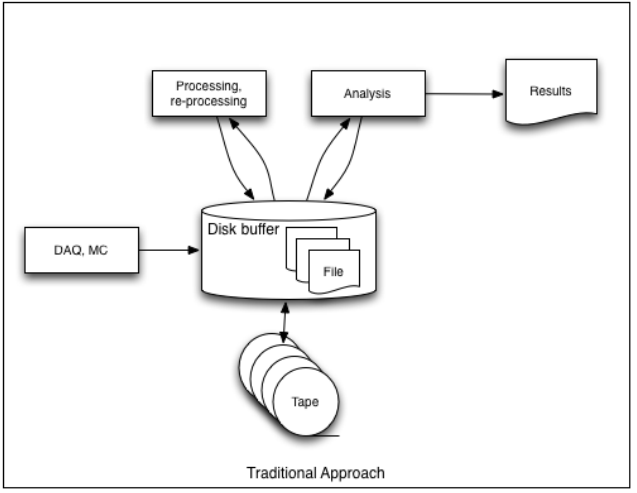
\includegraphics[height=0.42\textheight]{figures/production/traditional-data.png}
	\caption{A traditional approach to HEP data handling at FNAL~\cite{igor:bigdata}.}
	\label{fig:traditional-data}
\end{figure}
\begin{figure}
	\centering
	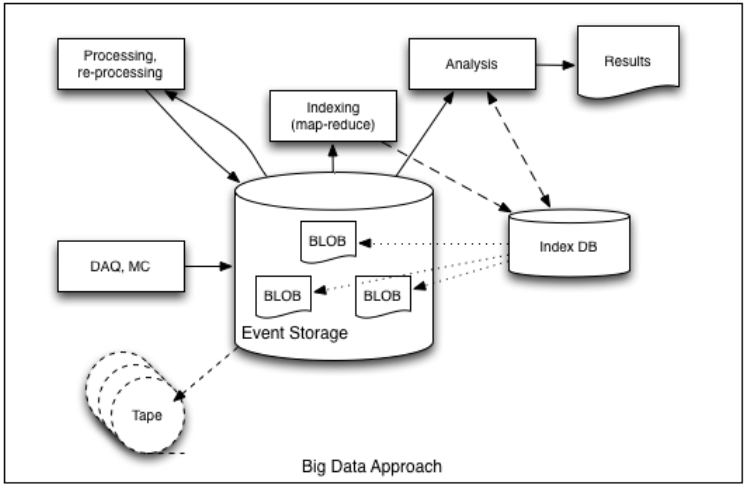
\includegraphics[height=0.355\textheight]{figures/production/new-proposal.png}
	\caption{A proposal that suggests using a combination of horizontally-scalable NoSQL technologies to store all data~\cite{igor:bigdata}. Blobs are ``binary large objects'' that are application-dependent -- they could be CODA or ROOT files, for instance.}
	\label{fig:big-data}
\end{figure}

In the proposal, Mandrichenko suggests using a NoSQL storage engine to store \emph{all} of the raw data from experiments at Fermilab combined with an SQL database to keep track of all of the indexing -- keep tabs of \emph{what} is in the mass storage and where to find it. The indexing engine can then be used by individuals/groups to index ``interesting'' data for their own analysis and can be summoned (even its raw data) at any time. In this paradigm, raw data is written to tape storage, but the philosophy here is ``write once, read hopefully never.'' Current estimates quote \unit[5]{PB} with 2-3x replication (effectively \unit[2]{PB}) storage) and an indexing server of $\sim$\unit[100]{TB}. This approach is laid out in visual detail in Figure~\ref{fig:big-data}. This proposal is simply an example of the type of technologies that are going to inevitably emerge as new facilities and experiments are put together.

Further into the future, though possibly sooner than one might imagine, cloud computing and storage has become more and more of a presence in both industry and academia. Not too long ago, it would have been almost unthinkable for a national laboratory or large industrial companies to store their data on server farms hosted by someone else. With the proliferation and maturity of Infrastructure-as-a-Service (IaaS) paradigm, services like Amazon Web Services (AWS), Microsoft Azure, and Google have truly emerged as a viable solution for institutions of all walks to trust them with their valuable data. Such providers are able to promptly provide scalable, ``elastic'' (expandable without downtime), redundant storage and processing using any storage engine, running on any operating system.

The matter simply comes down to the fact that assembling, administrating, and maintaining server hardware and systems has \emph{significant} overhead. Additionally, as technology evolves and new capabilities become possible, smaller operations become less agile in being able to keep up with developments as they happen. As IaaS providers have gradually earned the trust of users in the way of data security and redundancy, they have suddenly, over the past two years, become a \emph{leading} contender when new data infrastructure is considered.

When all costs are compared and needs are assessed, it would not surprise the author if mass data storage and handling are eventually outsourced to IaaS providers as new experiments are proposed in the next 5-\unit[10]{years}. The rationale behind this projection is that, since national labs and experiments are largely publicly funded, there will be pressure to spend the allotted funds in a responsible manner. As such services become cheaper, more effective, and more trusted, the number of reasons to keep data warehouses local to the laboratories will very quickly decline, and the pressure to adopt will increase.

There, however, will always be exceptions. In the cases of experiments like ATLAS and CMS, the data rates are beyond what exists elsewhere in the world at \unit[20+]{TB/day}~\cite{Andre:2015jty}. Clearly, for such situations, dedicated, specialized systems will likely need to be designed and maintained locally.
